\documentclass{article}

% if you need to pass options to natbib, use, e.g.:
% \PassOptionsToPackage{numbers, compress}{natbib}
% before loading nips_2017
%
% to avoid loading the natbib package, add option nonatbib:
% \usepackage[nonatbib]{nips_2017}


% to compile a camera-ready version, add the [final] option, e.g.:
% \usepackage[final]{nips_2017}

\usepackage[final]{nips_2018}

\usepackage{placeins}
\usepackage[utf8]{inputenc} % allow utf-8 input
\usepackage[T1]{fontenc}    % use 8-bit T1 fonts
\usepackage{hyperref}       % hyperlinks
\usepackage{url}            % simple URL typesetting
\usepackage{booktabs}       % professional-quality tables
\usepackage{amsfonts}       % blackboard math symbols
\usepackage{nicefrac}       % compact symbols for 1/2, etc.
\usepackage{microtype}      % microtypography
\usepackage{graphicx}

\title{COMP 4211 - Machine Learning Programming Assignment 1 Report}

\author{%
	Cheng Chi Fung \\
	\texttt{cfchengac@connect.ust.hk} \\
}

\begin{document}

\maketitle

\begin{abstract}
  In this assignment, we used linear regression, logistic regression and single layer neural network to perform the regression and classification on three binary classification and regression data sets.
  
\end{abstract}

\section{Linear Regression}

\subsection{Experienment Model Settings}

For linear regression, we used the built-in models   \textbf{LinearRegression} in skitlearn to perform the linear regression on three regression datasets .This model fits a linear model with coefficients  	$w = (w_1,..., w_p)$  to minimize the residual sum of squares between the observed responses in the dataset, and the responses predicted by the linear approximation. This model has \textbf{no hyperparameter} to set.

\begin{table}[htb]
	\caption{Experiments Datasets Settings}
	\label{sample-table}
	\centering
	\begin{tabular}{lll}
		\toprule
		\cmidrule{1-3}
		Dataset & Training set & Test set \\
		\midrule
		Fifa & $13191$ & $4397$ \\
		Finance & $2754$ & $918$ \\
		Orbits & $9642$ & $3215$ \\
		\bottomrule
	\end{tabular}
\end{table}

\subsection{Experiment Results}

The following are the experiment results which using the above model setting on fifa, finanace and orbits regression datasets.

\begin{table}[htb]
	\caption{Experiments Results of Linear Regression on Three Regression Datasets}
	\label{sample-table}
	\centering
	\begin{tabular}{lll}
		\toprule
		\cmidrule{1-3}
		\multicolumn{3}{c}{Coefficient of Determination ($R^2$ score)}\\
		\midrule
		Dataset & Training set & Test set \\
		\midrule
		Fifa & $0.51944$ & $0.51223$  \\
		Finance & $0.42637$  & $0.28766$ \\
		Orbits & $0.61671$  & $0.61016$  \\
		\bottomrule
	\end{tabular}
\end{table}

From the experiment results, we found out that excepts the \textbf{finance} datasets, the $R^2$ score of the training set and test set for the other twos are almost the same. And, for the finance datasets, the $R^2$ score of the test set ($0.42637$) are a much higher than the training set ($0.28766$). It means that this model  \textbf{overfit} the training data of the finance datasets.

\pagebreak

\begin{figure}[h]
  \centering
  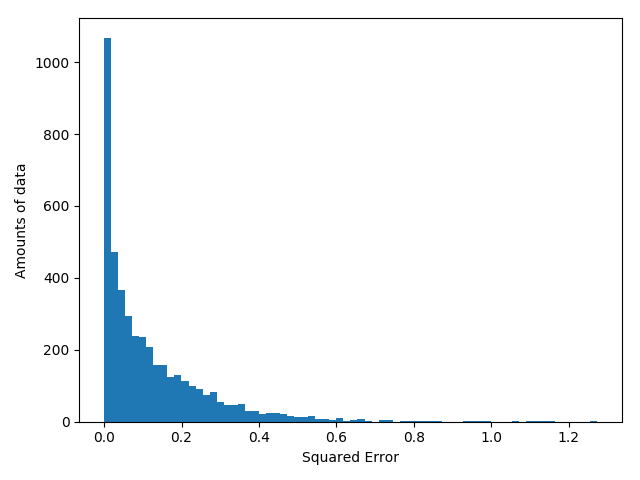
\includegraphics[scale=0.3]{fifa_lg.png}
  \caption{Squared Error Histogram on test set of orbits data set}
\end{figure}

\begin{figure}[h]
  \centering
  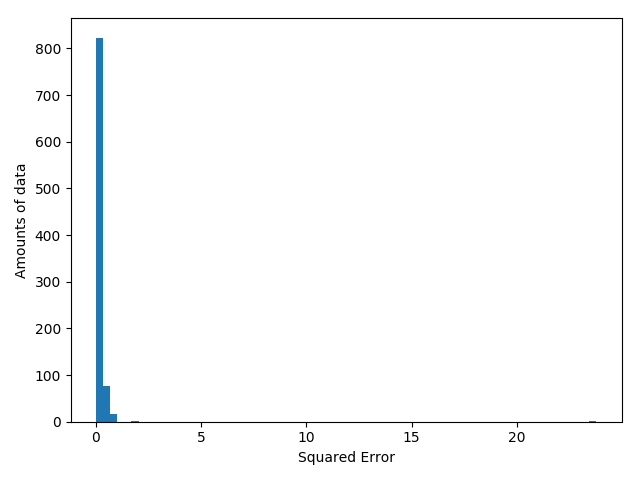
\includegraphics[scale=0.3]{finance_lg.png}
  \caption{Squared Error Histogram on test set of finance data set}
\end{figure}

\begin{figure}[h]
  \centering
  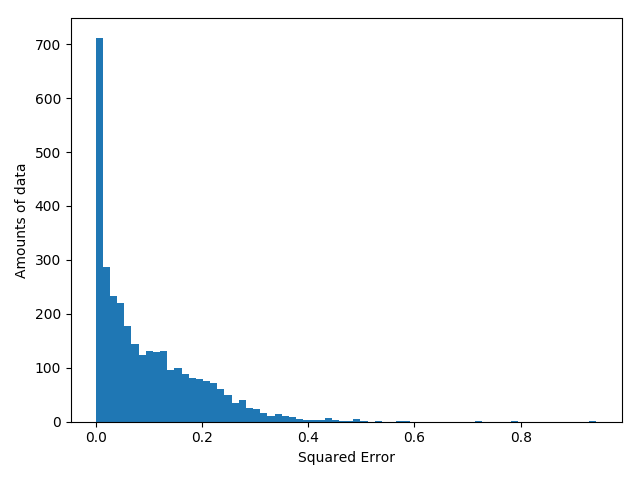
\includegraphics[scale=0.3]{orbit_lg.png}
  \caption{Squared Error Histogram on test set of orbit data set}
\end{figure}

From the square loss histogram of test sets, we found out that the mean squared error of the most of the data points are around zero. It means that this model perform quite well for most of the data points. However, for the finance datasets, there are some data points that have the sqaured error far away from zero ($23.77581$) which means that there might be some \textbf{outliers} that far away from the curve.

\pagebreak

\section{Logistic Regression}

\subsection{Experienmental Model Settings}

To perform the logistic regression with gradient-descent algorithm by minimizing the cross-entropy loss on the three classification datasets, we used the built-in model \textbf{SGDClassifier} in skitlearn. This model implements regularized linear models with \textbf{stochastic gradient descent} (SGD) learning. 


To get better training results, we first performed the \textbf{hyperparameters tunning} by using \textbf{GridSearchCV} in skitlearn to obtain best hyperparameters parameters on the training set of each datasets. The following are the settings for parameters tuning.

\begin{table}[htb]
	\caption{Model Settings for Hyperparameters Tuning (Tuned hyperparameters *)}
	\label{sample-table}
	\centering
	\begin{tabular}{lll}
		\toprule
		\cmidrule{1-2}
		Name     &  Parameter Setttings	\\
		\midrule
		max\_iter 		  & 	$5000$  \\
		learning\_rate 		  & 	optimal  \\
		loss 		  & 	log  \\
		tol      	          & 	  $0.000000001$        \\
		alpha* 		  & 	$0.1, 0.01,...,1^{-9}, 1^{-10}$    \\
		cv		  &   $5$     \\
		\bottomrule
	\end{tabular}
\end{table}

\begin{table}[htb]
	\caption{Best Hyperparameters after Hyperparameters Tuning}
	\label{sample-table}
	\centering
	\begin{tabular}{lll}
		\toprule
		\cmidrule{1-2}
		Dataset     &  alpha	\\
		\midrule
		fifa & $1^{-5}$  \\
		finance & $0.001$        \\
		orbits & $1^{-6}$ \\
		\bottomrule
	\end{tabular}
\end{table}



\subsection{Experiment Results}

The following are the experiment results which using the same setting as the hyperparameter tuning except the \textbf{alpha} using the best results after hyperparameters tuning on fifa, finanace and orbits classification datasets.

\begin{table}[htb]
	\caption{Experiments Results of Logistic Regression on Three Classification Datasets}
	\label{sample-table}
	\centering
	\begin{tabular}{lll}
		\toprule
		\cmidrule{1-3}
		\multicolumn{3}{c}{Classification Accuracy}\\
		\midrule
		Dataset & Training set & Test set \\
		\midrule
		Fifa & $0.82533$ & $0.81669$  \\
		Finance & $0.80355$  & $0.79084$ \\
		Orbits & $0.98610$  & $0.98755$  \\
		\bottomrule
	\end{tabular}
	\hspace{5mm}
	\centering
	\begin{tabular}{lll}
		\toprule
		\cmidrule{1-3}
		\multicolumn{3}{c}{AUC Score}\\
		\midrule
		Dataset & Training set & Test set \\
		\midrule
		Fifa & $0.93828$ & $0.93449$  \\
		Finance & $0.90664$  & $0.89185$ \\
		Orbits & $0.99995$  & $0.99992$  \\
		\bottomrule
	\end{tabular}
\end{table}

From the experiment results, we found out that the model perform \textbf{quite well} on three datasets which getting $>79\%$ on three datasets. However, its classification performace still \textbf{worse than single layer neural network} which will be disscussed in the next section. Furthermore, the better the AUC Score, the better the performace of the classifier. And from experiment results, we got a very high AUC score which mean that the model can classify the dataset very well.

\begin{figure}[h]
  \centering
  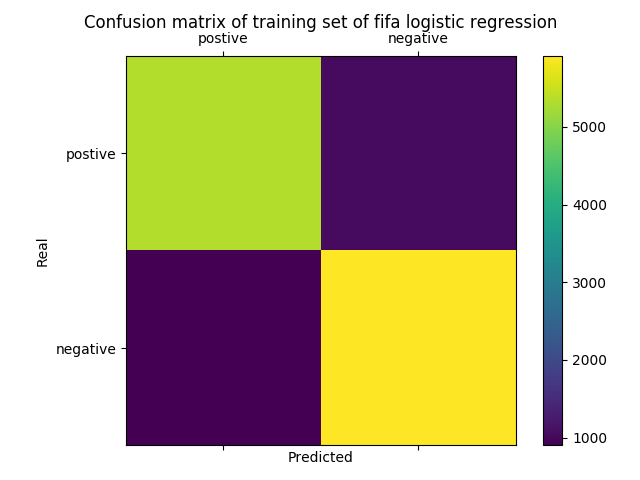
\includegraphics[scale=0.3]{fifa_lo_train.png}
  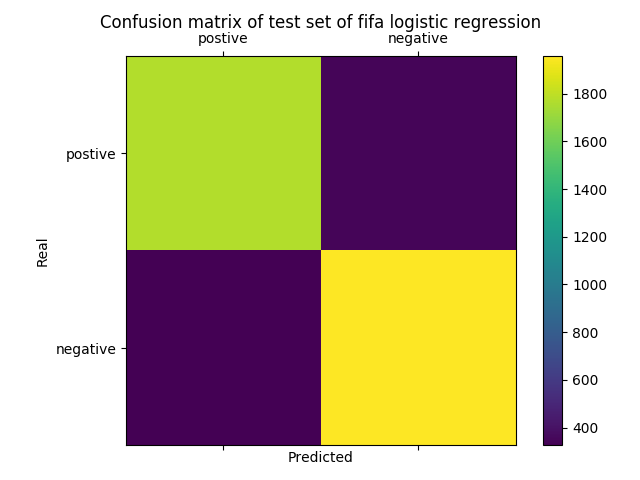
\includegraphics[scale=0.3]{fifa_lo_test.png}
  \caption{Confusion matrix of fifa data set}
\end{figure}

\FloatBarrier


\begin{figure}[h]
  \centering
  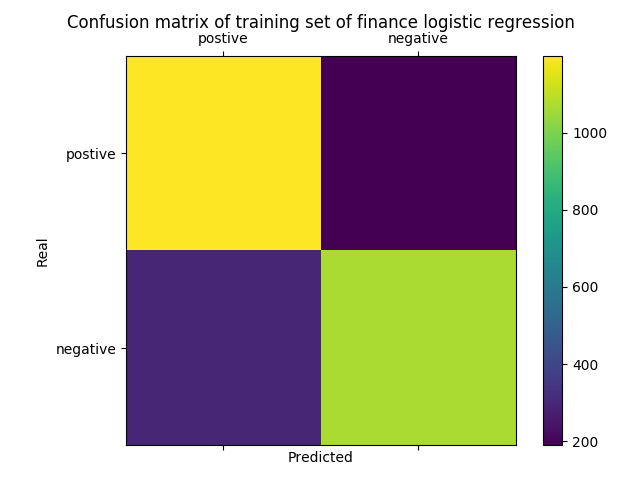
\includegraphics[scale=0.3]{finance_lo_train.png}
  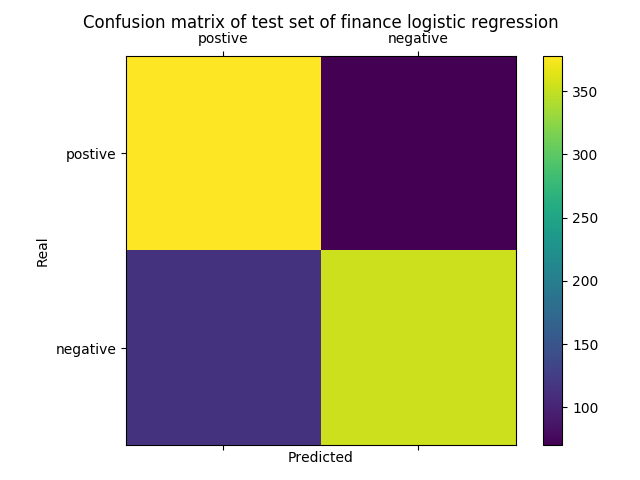
\includegraphics[scale=0.3]{finance_lo_test.png}
  \caption{Confusion matrix of finance data set}
\end{figure}

\begin{figure}[h]
  \centering
  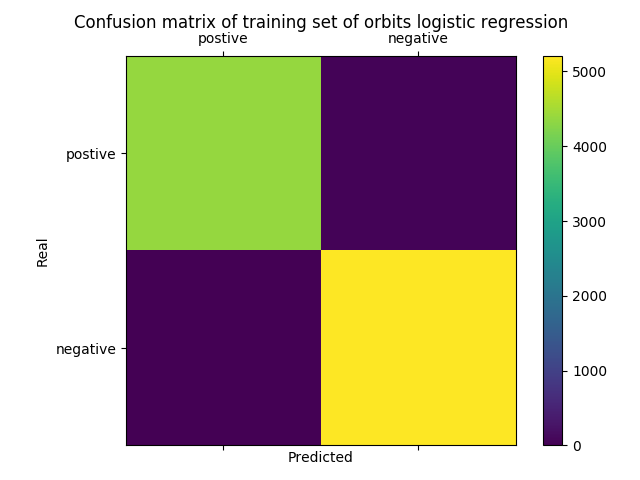
\includegraphics[scale=0.3]{orbits_lo_train.png}
  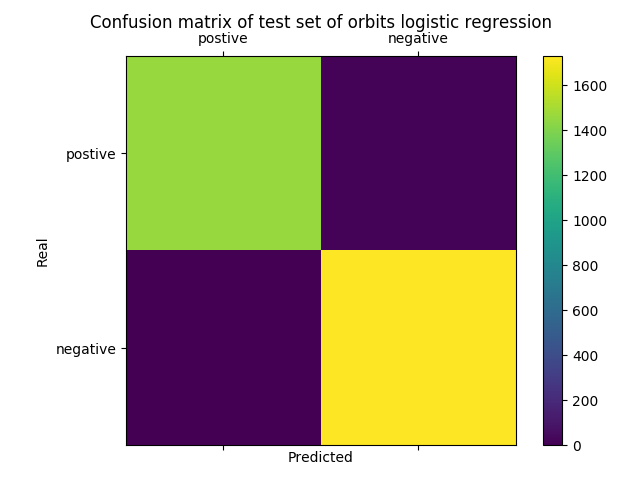
\includegraphics[scale=0.3]{orbits_lo_test.png}
  \caption{Confusion matrix of orbits data set}
\end{figure}

From the visulization of confusion matrix on three datasets, we found out that the model perform very well on both fifa and orbits dataset since there are deep purple color on the top right and the bottom left in the confusion matrix which means that it has \textbf{high true positive and true negative} rate during prediction. However, for the finance datasets, the bottom left purple color are not as deep as the other two which means that the prediction of this model on the finance datasets have a little bit higher \textbf{false postive} rate.

\begin{figure}[h]
  \centering
  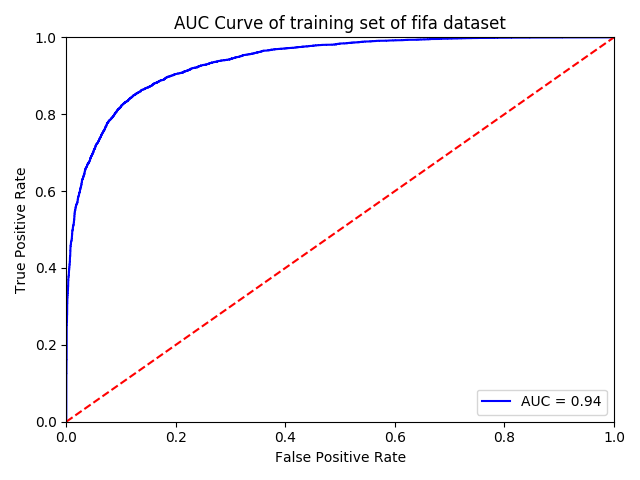
\includegraphics[scale=0.3]{fifa_auc_train.png}
  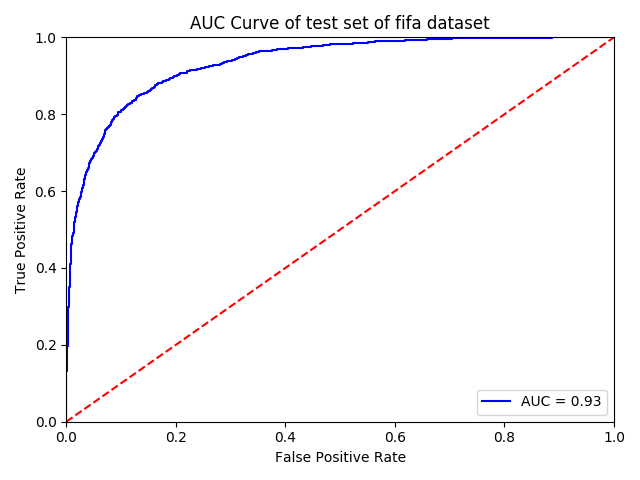
\includegraphics[scale=0.3]{fifa_auc_test.png}
  \caption{ROC curve of fifa data set}
\end{figure}

\FloatBarrier


\begin{figure}[h]
  \centering
  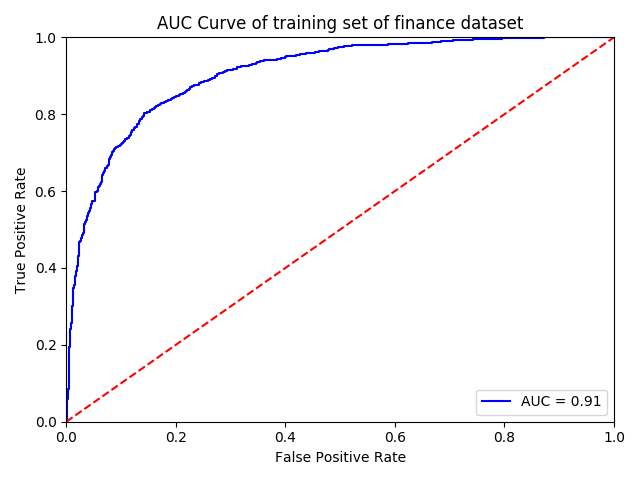
\includegraphics[scale=0.3]{finance_auc_train.png}
  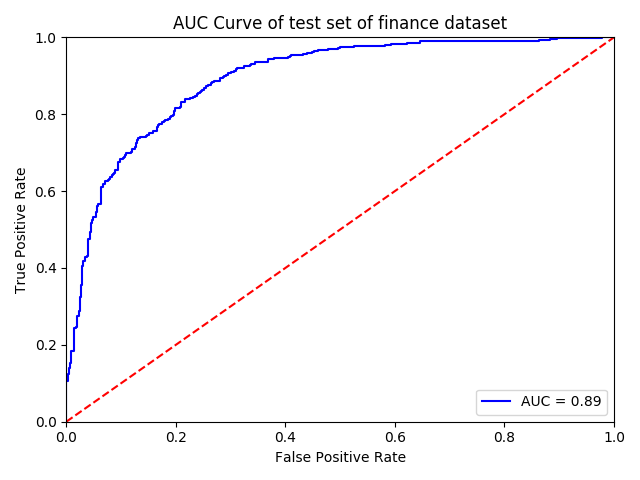
\includegraphics[scale=0.3]{finance_auc_test.png}
  \caption{ROC curve of finance data set}
\end{figure}

\begin{figure}[h]
  \centering
  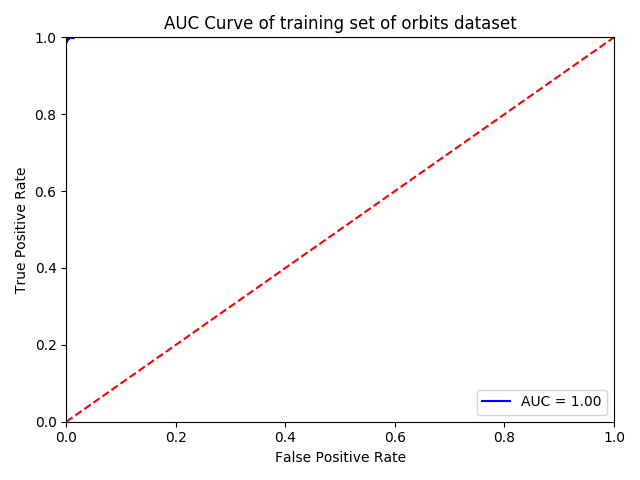
\includegraphics[scale=0.3]{orbits_auc_train.png}
  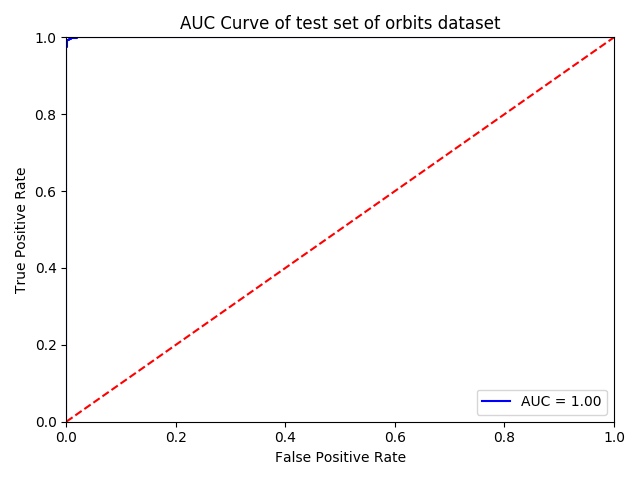
\includegraphics[scale=0.3]{orbits_auc_test.png}
  \caption{ROC curve of orbits data set}
\end{figure}

From the visulization of ROC Curve, since the curve are smooth on three datasets. Therefore, this model \textbf{does not overfit} the dataset.  

\pagebreak

\section{Single Layer Neural Network}

\subsection{Experienmental Model Settings}

To perform the classification with single layer neural network on the three classification datasets, we used the built-in model \textbf{MLPClassifier} in skitlearn. This model implements a multi-layer perceptron classifier and optimizes with the log-loss function using stochastic gradient descent.

To determine the number of \textbf{hidden units} should be used in the hidden layer, we evaludate the The generalization performance of the model with $i$ hidden units with \textbf{cross validation} (CV) using the utilities \textbf{cross\_val\_score} in skitlearn. The following are the model settings for cross validation and the results of that.

\begin{table}[htb]
	\caption{Model Settings for Cross Validation}
	\label{sample-table}
	\centering
	\begin{tabular}{lll}
		\toprule
		\cmidrule{1-2}
		Name     &  Parameter Setttings	\\
		\midrule
		max\_iter & $5000$  \\
		learning\_rate & optimal  \\
		solver & sgd  \\
		tol & $0.000000001$        \\
		alpha & determined by using grid search for each $i$ hidden unit   \\
		cv & $5$     \\
		\bottomrule
	\end{tabular}
\end{table}

\begin{table}[htb]
	\caption{Performance of the Model with $i$ Hidden Units using Cross Validation}
	\label{sample-table}
	\centering
	\begin{tabular}{lll}
		\toprule
		\cmidrule{1-2}
		$i$ hidden units    &  Score (Average Classification Accuracy)	\\
		\cmidrule{1-2}
		 &  Fifa, Finance, Orbits	\\
		\midrule
		1 & $0.65346$, $0.67176$, $0.99398$ \\
		2 & $0.86142$, $0.68424$, $0.90243$ \\
		3 & $0.86028$, $0.80501$, $0.99429$ \\
		4 & $0.86119$, $0.80647$, $0.99367$ \\
		5 & $0.86089$, $0.80464$, $0.99367$ \\
		6 & $0.85869$, $0.80900$, $0.99336$ \\
		7 & $0.85975$, $0.80247$, $0.99398$ \\
		8 & $0.86020$, $0.80501$, $0.99387$ \\
		9 & $0.86134$, $0.80429$, $0.99419$ \\
		10 & $0.86088$, $0.80320$, $0.99263$ \\
		\midrule
		Number of hidden units with highest score & $2 (0.86142)$, $6 (0.80900)$, $3 (0.99429)$ \\
		\bottomrule
	\end{tabular}
\end{table}

Furthermore, to \textbf{avoid overfitting}, we performed the parameters tuning on the \textbf{number of iterations} after getting the best number of hidden units with cross validation. The model settings for parameters tuning 
used the same model settings as cross validation and the number hidden units using what we got from cross validation. We tuned the number of iteraion by returning the maximum iterations before loss of the test set start to decrease. 

\begin{table}[htb]
	\caption{Model Settings for Parameter Tuning(Tuned hyperparameters *)}
	\label{sample-table}
	\centering
	\begin{tabular}{lll}
		\toprule
		\cmidrule{1-2}
		Name     &  Parameter Setttings	\\
		\midrule
		max\_iter* & $1000,1500,2000,...,8000,8500$  \\
		learning\_rate & optimal  \\
		solver & sgd  \\
		tol & $0.000000001$        \\
		alpha & determined by using grid search before   \\
		hidden units & determined by using CV before     \\
		\bottomrule
	\end{tabular}
\end{table}

\pagebreak

\begin{table}[htb]
	\caption{Best Hyperparameters after Hyperparameters Tuning}
	\label{sample-table}
	\centering
	\begin{tabular}{lll}
		\toprule
		\cmidrule{1-2}
		Dataset     &  max\_iter	\\
		\midrule
		fifa & $1000$  \\
		finance & $4500$        \\
		orbits & $8000$ \\
		\bottomrule
	\end{tabular}
\end{table}

After hyperparameters tuning on number of iterations, we obtain the best \textbf{max\_iteration} before overfitting to the training set. Finally, we got the following model settings for our final training.

\begin{table}[h]
	\caption{Model Settings of Using Single Layer Nerual Network }
	\label{sample-table}
	\centering
	\begin{tabular}{lll}
		\toprule
		\cmidrule{1-2}
		Name     &  Parameter Setttings	\\
		\cmidrule{1-2}
		 &  Fifa, Finance, Orbits	\\
		\midrule
		max\_iter & $1000$, $1000$, $1500$  \\
		learning\_rate & optimal \\
		solver & sgd \\
		tol & $0.000000001$ \\
		alpha & $0.0001$, $1^{-9}$, $0.01$   \\
		number of hidden units & $2$, $6$, $3$    \\
		\bottomrule
	\end{tabular}
\end{table}



\subsection{Experienment Results}

The following are the experiment results which using the above model setting on fifa, finanace and orbits classification datasets.

\begin{table}[htb]
	\caption{Experiments Results of Logistic Regression on Three Classification Datasets}
	\label{sample-table}
	\centering
	
		\begin{tabular}{lll}
		\toprule
		\cmidrule{1-3}
		\multicolumn{3}{c}{Classification Accuracy}\\
		\midrule
		Dataset & Training set & Test set \\
		\midrule
		Fifa & $0.93828$ & $0.93449$  \\
		Finance & $0.82933$  & $0.80718$ \\
		Orbits & $0.99533$  & $0.99502$  \\
		\bottomrule
	\end{tabular}
	
		\begin{tabular}{lll}
		\toprule
		\cmidrule{1-3}
		\multicolumn{3}{c}{Loss}\\
		\midrule
		Dataset & Training set & Test set \\
		\midrule
		Fifa & $0.31560$ & $0.32098$  \\
		Finance & $0.38444$  & $0.39380$ \\
		Orbits & $0.07369$  & $0.05241$  \\
		\bottomrule
	\end{tabular}
	\hspace{5mm}
	\begin{tabular}{lll}
		\toprule
		\cmidrule{1-3}
		\multicolumn{3}{c}{AUC Score}\\
		\midrule
		Dataset & Training set & Test set \\
		\midrule
		Fifa & $0.94828$ & $0.93449$  \\
		Finance & $0.91933$  & $0.89718$ \\
		Orbits & $0.99997$  & $0.99995$  \\
		\bottomrule
	\end{tabular}
	

\end{table}

From the experiment results, we found out that the single layer neural network \textbf{perform better than logistic regression} which has higher classification accuracy on three datasets. And the loss of the training set and test set are similiar which means that the model are \textbf{not overfit} to the training data set. And for the AUC score, single layer neural network perform slightly better than logistic.

\begin{figure}[h]
  \centering
  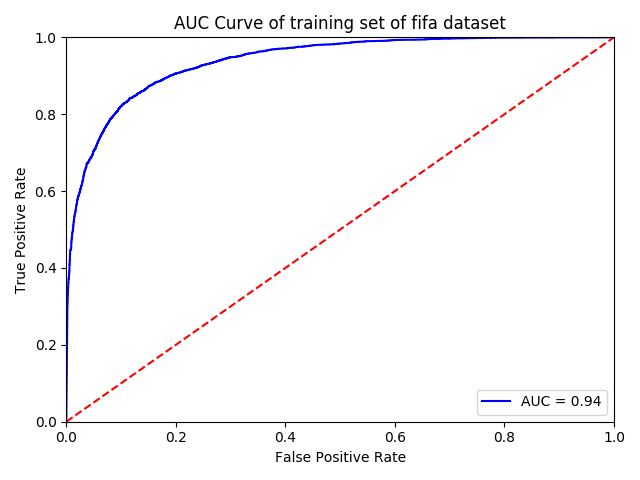
\includegraphics[scale=0.3]{auc_fifa_train.png}
  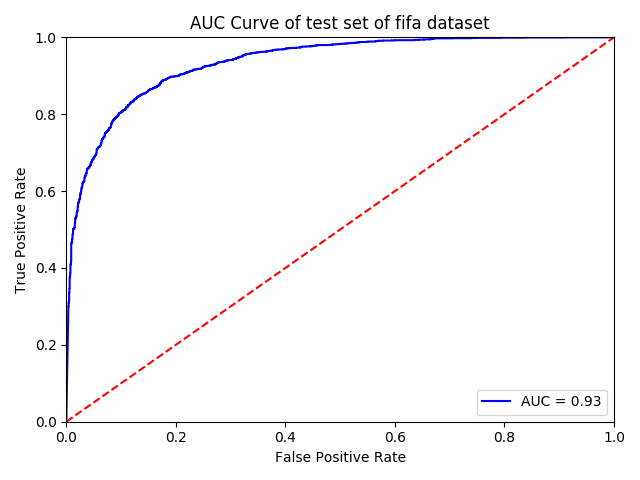
\includegraphics[scale=0.3]{auc_fifa_test.png}
  \caption{ROC curve of fifa data set}
\end{figure}

\FloatBarrier


\begin{figure}[h]
  \centering
  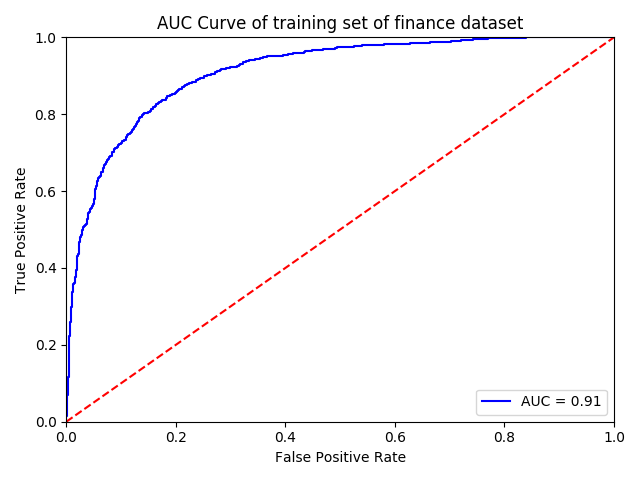
\includegraphics[scale=0.3]{auc_finance_train.png}
  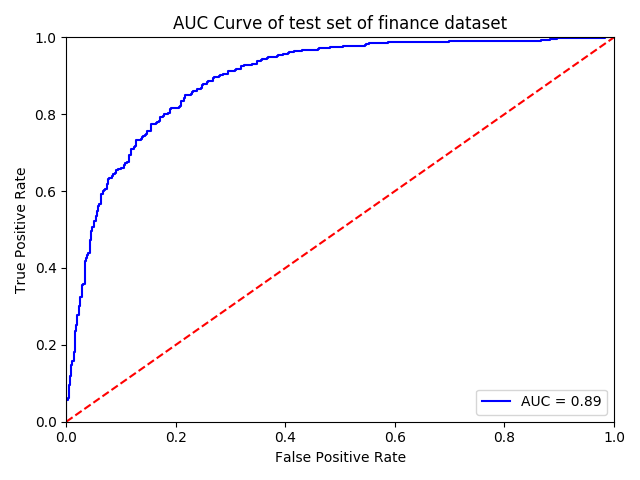
\includegraphics[scale=0.3]{auc_finance_test.png}
  \caption{ROC curve of finance data set}
\end{figure}

\begin{figure}[h]
  \centering
  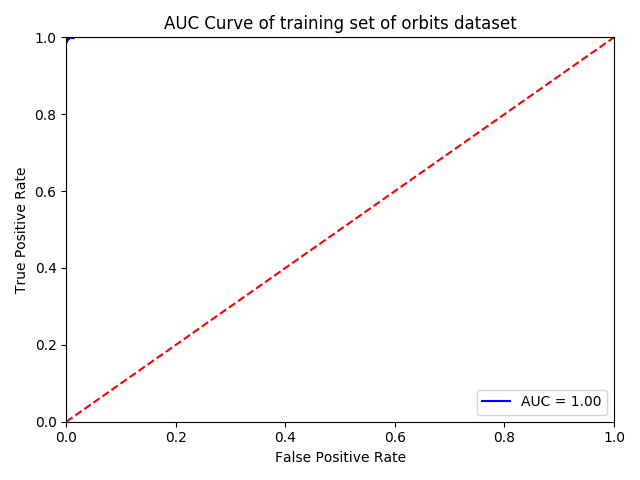
\includegraphics[scale=0.3]{orbits_auc_train.png}
  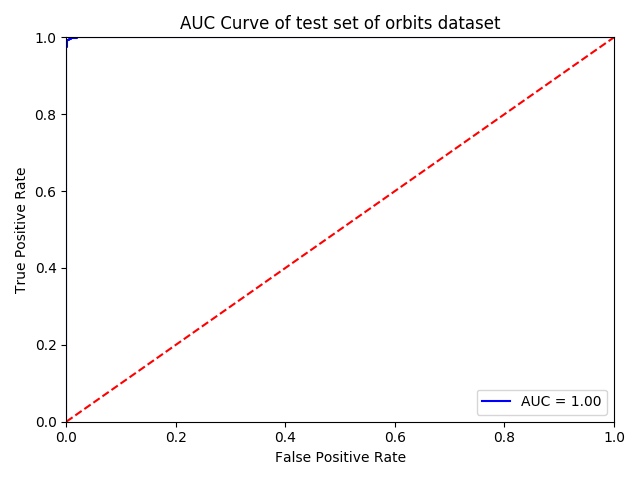
\includegraphics[scale=0.3]{orbits_auc_test.png}
  \caption{ROC curve of orbits data set}
\end{figure}

From the visulization of ROC Curve, since the curve are smooth on three datasets. Therefore, this model \textbf{does not overfit} the dataset.  

\pagebreak

The following are the visualization of the peroformace during training. (Y axis = loss / X axis = iterations)

\begin{figure}[h]
  \centering
  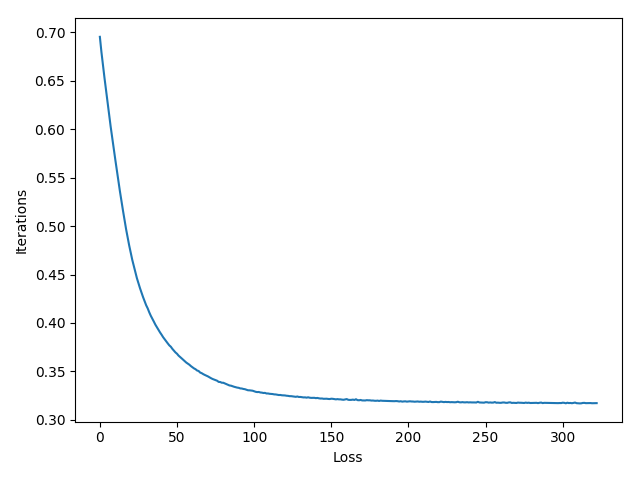
\includegraphics[scale=0.3]{loss_fifa.png}
  \caption{Loss curve of train set of fifa data set}
\end{figure}

\begin{figure}[h]
  \centering
  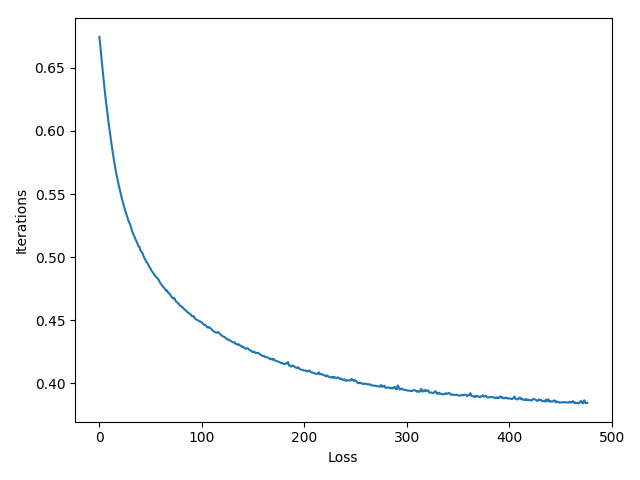
\includegraphics[scale=0.3]{loss_finance.png}
  \caption{Loss curve of train set of finance data set}
\end{figure}

\begin{figure}[h]
  \centering
  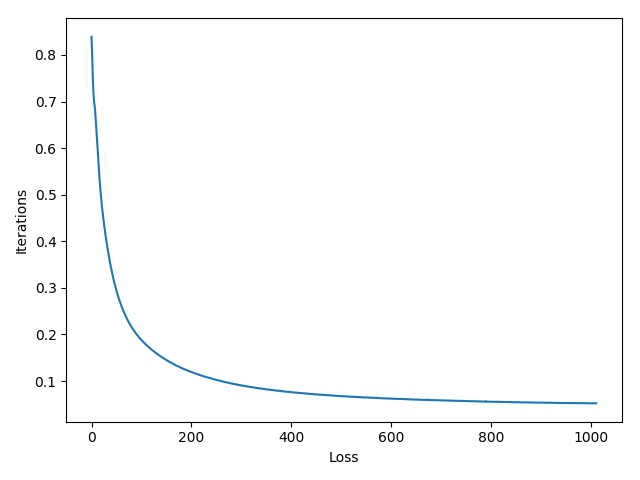
\includegraphics[scale=0.3]{loss_orbits.png}
  \caption{Loss curve of train set of orbits data set}
\end{figure}


\pagebreak

\section{Computing Environment and Time Used}

\subsection{Computing Environment}

\begin{table}[htb]
	\caption{Computing Environment}
	\label{sample-table}
	\centering
	\begin{tabular}{lll}
		\toprule
		\cmidrule{1-2}
		    &  Environment Settings	\\
		\midrule
		CPU & AMD Ryzen™ 7 2700X   \\
		GPU & GTX 1080Ti        \\
		RAM & 16GB \\
		STORAGE & 1TB M2 NVME SSD \\
		OS & Ubuntu 16.04 \\
		IDE & Pycharm \\
		Python Version & Python 3.5.2 \\
		Libraries Used & skitlearn, numpy, matplotlib.pyplot \\
		\bottomrule
	\end{tabular}
\end{table}

\subsection{Time Used}

\begin{table}[htb]
	\caption{Total Running Time For Each Tasks}
	\label{sample-table}
	\centering
	\begin{tabular}{lll}
		\toprule
		\cmidrule{1-2}
		    &  Wall Time	(seconds)\\
		\midrule
		Linear Regression & $0.470023$ \\
		Logistic Regression & $10.86583$ \\
		Single Layer Neural Network & $8376.50412$ \\
		\bottomrule
	\end{tabular}
\end{table}

\end{document}

